
\chapter[Bài tập: Điều kiện xảy ra sóng dừng và hình dạng sóng dừng;\\Bài tập: Dao động của các phần tử trong sóng dừng]{Bài tập: Điều kiện xảy ra sóng dừng và hình dạng sóng dừng;\\Bài tập: Dao động của các phần tử trong sóng dừng}
\section{Lý thuyết}
\subsection{Sóng dừng trên sợi dây có hai đầu cố định}
\subsubsection{Hình dạng sóng dừng trên sợi dây có hai đầu cố định}
\begin{center}
	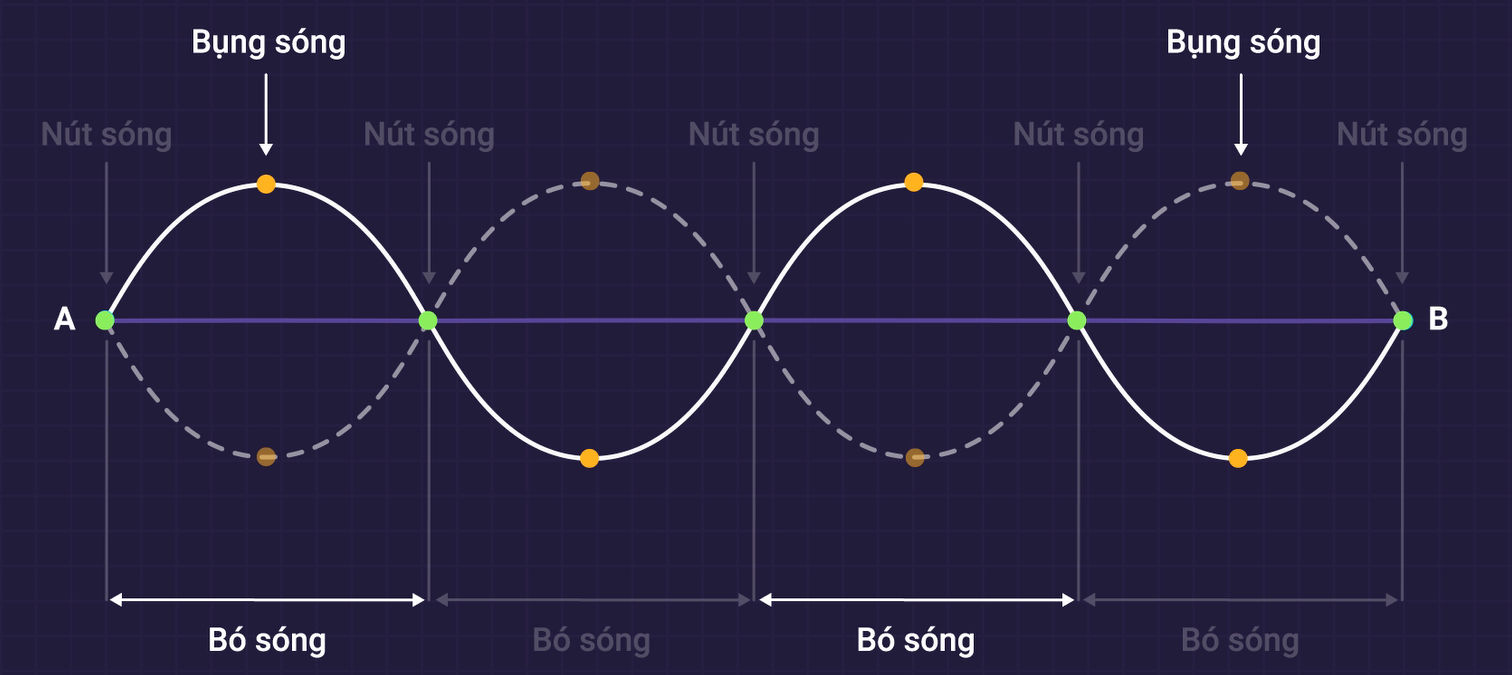
\includegraphics[scale=0.35]{../figs/VN12-PH-12-A-008-1-V2-1.png}
\end{center}
\subsubsection{Điều kiện xảy ra sóng dừng trên sợi dây có hai đầu cố định}
Điều kiện để có sóng dừng trên một sơi dây có hai đầu cố định là chiều dài của sợi dây phải bằng một số nguyên lần nửa bước sóng:
\begin{equation*}
	l=k\dfrac{\lambda}{2}\qquad(k=1,2,3,\ldots);
\end{equation*}
trong đó: $k$ là số bó sóng nguyên.

\begin{center}
	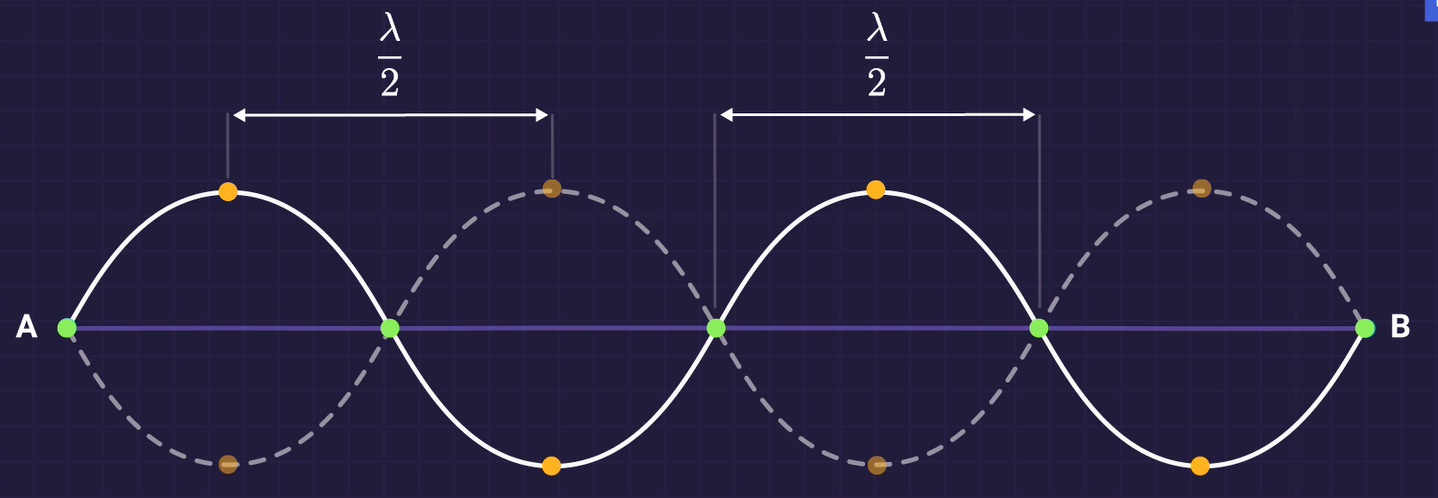
\includegraphics[scale=0.4]{../figs/VN12-PH-12-A-008-1-V2-2.png}
\end{center}
\luuy{Công thức trên cũng đúng với trường hợp sợi dây có hai đầu tự do.}
\subsection{Sóng dừng trên sợi dây có một đầu cố định, một đầu tự do}
Điều kiện để có sóng dừng trên một sơi dây có một đầu cố định, một đầu tự do là chiều dài của sợi dây phải bằng một số lẻ lần $\dfrac{\lambda}{4}$
\begin{equation*}
	l=(2k+1)\dfrac{\lambda}{4},\qquad(k=0,1,2,3,\ldots),
\end{equation*}
trong đó: $k$ là số bó sóng nguyên.
\begin{center}
	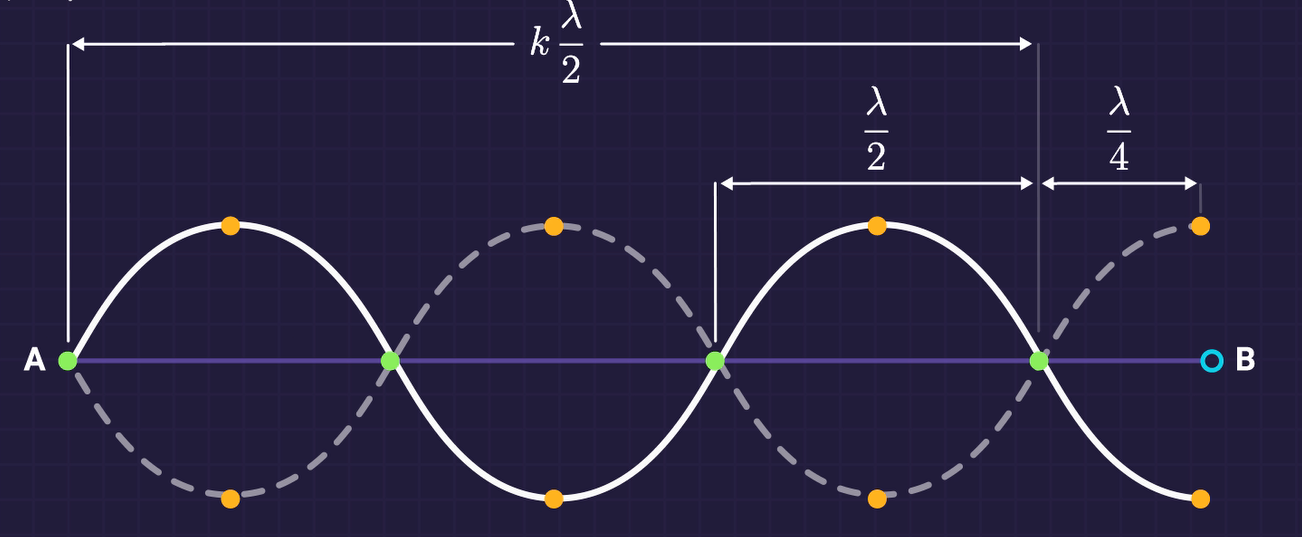
\includegraphics[scale=0.4]{../figs/VN12-PH-12-A-008-1-V2-3.png}
\end{center}
\luuy{
	\begin{itemize}
		\item Nếu một đầu dây được gắn với âm thoa để tạo sóng dừng thì đầu dây đó luôn là nút sóng.
		\item Đầu cố định hoặc đầu dao động nhỏ là nút sóng. Đầu tự do là bụng sóng.
		\item Khoảng cách gần nhất giữa hai bụng sóng (hoặc hai nút sóng) là $\lambda/2$.
		\item Khoảng cách gần nhất giữa một nút sóng và một bụng sóng là $\lambda/4$.
		\item Khoảng thời gian ngắn nhất giữa hai lần sợi dây duỗi thẳng là $T/2$.
\end{itemize}}
\subsection{Dao động trên sợi dây kim loại bị kích thích bởi nam châm điện}
\begin{itemize}
	\item Sợi dây \textbf{không} có dòng điện chạy qua, sóng dừng được tạo bởi sự rung của nam châm điện có tần số $f$ thì tần số dao động của sợi dây là $2f$.
	\item Sợi dây \textbf{có} dòng điện chạy qua, sóng dừng được tạo bởi sự rung của nam châm điện và dòng điện có tần số $f$ thì tần số dao động của sợi dây là $f$.
\end{itemize}
\subsection{Phương trình sóng dừng}
\subsubsection{Đầu B cố định (B là nút sóng)}

Phương trình sóng tới và sóng phản xạ tại B là
\begin{equation*}
	\begin{cases}
		u_\text{B}=A\cos \omega t \\ 
		u_\text{B}'=A\cos (\omega t-\pi).
	\end{cases}
\end{equation*}

Phương trình sóng dừng tại điểm M bất kì trên dây:
\begin{equation*}
	u_\text{M}=2A\sin\left( \dfrac{2\pi d}{\lambda}\right) \sin\omega t = 2A\sin\left( \dfrac{2\pi d}{\lambda}\right) \cos\left( \omega t - \dfrac{\pi}{2}\right). 
\end{equation*}

Biên độ sóng dừng tại một điểm M cách đầu cố định B (hoặc cách một nút sóng bất kì) một khoảng $d$ là
\begin{equation*}
	A_\text{M}=2A\left|\sin\left( \dfrac{2\pi d}{\lambda}\right)\right| = A_\text{b}\left|\sin\left( \dfrac{2\pi d}{\lambda}\right)\right|,
\end{equation*}
với $A_\text{b}$ là biên độ của bụng sóng.

\subsubsection{Đầu B tự do (B là bụng sóng)}

Phương trình sóng tới và sóng phản xạ trên dây là
\begin{equation*}
	\begin{cases}
		u_\text{B}=A\cos \omega t \\ 
		u_\text{B}'=A\cos \omega t.
	\end{cases}
\end{equation*}

Phương trình sóng dừng tại điểm M bất kì trên dây:
\begin{equation*}
	u_\text{M}=2A\sin\left( \dfrac{2\pi d}{\lambda}\right) \cos\omega t. 
\end{equation*}

Biên độ sóng dừng tại một điểm M cách đầu tự do B (hoặc cách một nút sóng bất kì) một khoảng $d$ là
\begin{equation*}
	A_\text{M}=2A\left|\cos\left( \dfrac{2\pi d}{\lambda}\right)\right| = A_\text{b}\left|\cos\left( \dfrac{2\pi d}{\lambda}\right)\right|,
\end{equation*}
với $A_\text{b}$ là biên độ của bụng sóng.		

\luuy{
	\begin{itemize}
		\item Biên độ của bụng sóng bằng $A_\text{b}=2A$.
		\item Bề rộng của bụng sóng bằng $4A$.
	\end{itemize}
}
\section{Mục tiêu bài học - Ví dụ minh họa}
\begin{dang}{Ghi nhớ được các điều kiện\\ để có sóng dừng}
	\viduii{1}
	{Sóng truyền trên sợi dây đàn hồi có hai đầu cố định với bước sóng $\lambda$. Để trên dây có sóng dừng thì chiều dài của sợi dây bằng
		\begin{mcq}(2)
			\item $(2k+1)\dfrac{\lambda}{2}$ với $k=0; 1; 2; \ldots$
			\item $k \dfrac{\lambda}{2}$ với $k=1; 2;3; \ldots$
			\item $(2k+1) \dfrac{\lambda}{4}$ với $k=0; 1; 2; \ldots$
			\item $(2k+1)\dfrac{\lambda}{2}$ với $k=1; 2; 3; \ldots$
		\end{mcq}
	}
	{
		\begin{center}
			\textbf{Hướng dẫn giải}
		\end{center}
		
		Để trên dây đàn hồi có hai đầu cố định có sóng dừng thì chiều dài của sợi dây $$L=k \dfrac{\lambda}{2},$$ với $k=1; 2;3; \ldots$
		
		\textbf{Đáp án: B.}
	}
	\viduii{1}
	{Điều kiện để có sóng dừng trên một sơi dây có $\ldots$ là chiều dài của sợi dây phải bằng một số lẻ lần $\dfrac{\lambda}{4}$. Hãy tìm cụm từ thích hợp điền vào chỗ trống.
		
		\begin{mcq}(2)
			\item hai đầu cố định
			\item hai đầu tự do
			\item một đầu cố định, một đầu tự do
			\item hai đầu không cố định
		\end{mcq}
	}
	{\begin{center}
			\textbf{Hướng dẫn giải}
		\end{center}
		
		Điều kiện để có sóng dừng trên một sơi dây có một đầu cố định, một đầu tự do là chiều dài của sợi dây phải bằng một số lẻ lần $\dfrac{\lambda}{4}$.
		
		\textbf{Đáp án: C.}
	}
\end{dang}
\begin{dang}{Sử dụng được điều kiện sóng dừng\\ để xác định chiều dài sợi dây, vận tốc truyền sóng, tần số, $\ldots$}
	\viduii{3}
	{Quan sát sóng dừng trên một sợi dây đàn hồi, người ta đo được khoảng cách giữa 5 nút sóng liên tiếp là 100 cm. Biết tần số của sóng truyền trên dây là 100 Hz. Vận tốc truyền sóng trên dây là
		\begin{mcq}(4)
			\item 50 m/s.
			\item 100 m.s. 
			\item 25 m/s.
			\item 75 m/s.
		\end{mcq}
	}
	{
		\begin{center}
			\textbf{Hướng dẫn giải}
		\end{center}
		
		Khoảng cách giữa 5 nút sóng liên tiếp trên sợi dây có sóng dừng:
		$$100\ \text{cm} = 4 \dfrac{\lambda}{2} \Rightarrow \lambda = 0,5\ \text{m}.$$
		
		Vận tốc truyền sóng:
		$$v=\lambda f = 50\ \text{m/s}.$$
		
		\textbf{Đáp án: A.}
	}
	\viduii{3}
	{Một sợi dây căng ngang giữa hai điểm cố định cách nhau $75\ \text{cm}$. Người ta tạo sóng dừng trên dây. Hai tần số gần nhau nhất cùng tạo ra sóng dừng trên dây là $150\ \text{Hz}$ và $200\ \text{Hz}$. Tần số nhỏ nhất tạo ra sóng dừng trên dây đó là
		\begin{mcq}(4)
			\item $100\ \text{Hz}$.
			\item $125\ \text{Hz}$.
			\item $75\ \text{Hz}$.
			\item $50\ \text{Hz}$.
		\end{mcq}	
	}
	{\begin{center}
			\textbf{Hướng dẫn giải}
		\end{center}
		
		Tần số tạo sóng dừng được suy ra từ điều kiện xảy ra sóng dừng:
		$$l=k\dfrac{\lambda}{2}=k\dfrac{v}{2f}\Rightarrow f=\dfrac{kv}{2l}.$$
		Công thức trên cho thấy tần số $f$ nhỏ nhất ứng với giá trị $k$ nhỏ nhất ($k=1$), do đó 
		$$f_\text{min} = \dfrac{1\cdot v}{2l}=\dfrac{(k+1)v}{2l} - \dfrac{kv}{2l} = \SI{50}{\hertz}.$$
		
		\textbf{Đáp án: D.}	
	}
	\viduii{3}
	{Một sợi dây đàn hồi dài $\SI{90}{cm}$ có một đầu cố định và một đầu tự do đang có sóng dừng. Kể cả đầu cố định, trên dây có 8 nút. Biết rằng khoảng thời gian giữa 6 lần liên tiếp sợi dây duỗi thẳng là $\SI{0.25}{\second}$. Tốc độ truyền sóng trên dây là
		\begin{mcq}(4)
			\item $\SI{1.2}{\meter/\second}$.
			\item $\SI{2.9}{\meter/\second}$.
			\item $\SI{2.4}{\meter/\second}$.
			\item $\SI{2.6}{\meter/\second}$.
		\end{mcq}
	}
	{
		\begin{center}
			\textbf{Hướng dẫn giải}
		\end{center}
		
		Khoảng thời gian giữa 6 lần liên tiếp sợi dây duỗi thẳng là $\SI{0.25}{\second}$ nên
		$$5\cdot\dfrac{T}{2}=\SI{0.25}{\second}\Rightarrow T=\SI{0.1}{\second}.$$
		
		Dây có một đầu cố định và một đầu tự do đang có sóng dừng, kể cả đầu cố định, trên dây có 8 nút nên
		$$l=7\cdot\dfrac{\lambda}{2}+\dfrac{\lambda}{4}=\SI{0.9}{\meter}\Rightarrow\lambda=\SI{0.24}{\meter}.$$
		
		Tốc độ truyền sóng trên dây là
		$$v=\dfrac{\lambda}{T}=\dfrac{\SI{0.24}{\meter}}{\SI{0.1}{\second}}=\SI{2.4}{\meter/\second}.$$
		
		\textbf{Đáp án: C.}}
\end{dang}
\begin{dang}{Xác định được số bụng, số nút\\ trên sợi dây có sóng dừng}
	\viduii{3}
	{Trên một sợi dây đàn hồi dài có sóng dừng với bước sóng $\SI{1.4}{cm}$. Trên dây có hai điểm A và B cách nhau $\SI{5.6}{cm}$. Biết A, B là một bụng. Số nút sóng và bụng sóng trên đoạn dây AB là
		\begin{mcq}(2)
			\item 8 nút và 9 bụng.
			\item 9 nút và 8 bụng.
			\item 9 nút và 10 bụng.
			\item 10 nút và 9 bụng.
		\end{mcq}
	}
	{
		\begin{center}
			\textbf{Hướng dẫn giải}
		\end{center}
		
		Ta có: A,B là bụng sóng và $\text{AB}=4\lambda=8\dfrac{\lambda}{2}.$
		
		$\Rightarrow $ Trên dây AB có 8 nút sóng và 9 bụng sóng.
		
		\textbf{Đáp án: A.}
	}
	\viduii{3}
	{Một sợi dây MN dài $\SI{150}{\centi\meter}$ căng ngang, đầu N cố định, đầu M gắn với một nhánh của âm thoa dao động điều hòa với tần số $\SI{40}{\hertz}$. Trên dây MN có một sóng dừng ổn định, M được coi là nút sóng. Tốc độ truyền sóng trên dây là $\SI{20}{\meter/\second}$. Kể cả M và N, trên dây có
		\begin{mcq}(2)
			\item 7 nút và 6 bụng.
			\item 6 nút và 7 bụng.
			\item 7 nút và 7 bụng.
			\item 6 nút và 6 bụng.
		\end{mcq}
	}
	{
		\begin{center}
			\textbf{Hướng dẫn giải}
		\end{center}
		
		Bước sóng trên dây MN là
		\begin{equation*}
			\lambda=\frac{v}{f}=\frac{\SI{20}{\meter/\second}}{\SI{40}{\hertz}}=\SI{0,5}{\meter}.
		\end{equation*}
		
		Vì M, N là nút nên
		\begin{equation*}
			d=k\frac{\lambda}{2}\Rightarrow \SI{1,5}{\meter}=k\frac{\SI{0,5}{\meter}}{2}\Rightarrow k=6.
		\end{equation*}
		
		Vì $k=6$, nên trên dây MN có 6 bó sóng nguyên và M và N là nút và nên kể cả M và N có 6 bụng và 7 nút.
		
		\textbf{Đáp án: A.}
	}
	\viduii{3}
	{Một sợi dây đàn hồi dài $\SI{90}{\centi\meter}$ có một đầu cố định và một đầu tự do đang có sóng dừng. Biết rằng khoảng thời gian giữa 6 lần liên tiếp sợi dây duỗi thẳng là $\SI{0,25}{\second}$, tốc độ truyền sóng trên dây là $\SI{2,4}{\meter/\second}$. Kể cả đầu cố định, trên dây có
		\begin{mcq}(2)
			\item 8 nút và 8 bụng.
			\item 7 nút và 8 bụng.
			\item 8 nút và 7 bụng.
			\item 7 nút và 7 bụng.
		\end{mcq}
	}
	{\begin{center}
			\textbf{Hướng dẫn giải}
		\end{center}
		
		Khoảng thời gian giữa 6 lần liên tiếp sợi dây duỗi thẳng là $0,25\ \text s$ nên:
		\begin{equation*}
			5\cdot\frac{T}{2}=\SI{0,25}{\second}\Rightarrow T = \SI{0,1}{\second}.
		\end{equation*}
		
		Bước sóng trên dây là
		\begin{equation*}
			\lambda=\frac{v}{f}=v\cdot T=\SI{2,4}{\meter/\second}\cdot \SI{0,1}{\second}=\SI{0,24}{\meter}.
		\end{equation*}
		
		Vì sợi dây có một đầu cố định, một đầu tự do nên
		\begin{equation*}
			d=(2k+1)\frac{\lambda}{4}\Rightarrow \SI{0,9}{\meter}=(2k+1)\frac{\SI{0,24}{\meter}}{4}\Rightarrow k=7.
		\end{equation*}
		
		Vì sợi dây có một đầu cố định, một đầu tự do và $k=7$ nên trên dây có 7 bó sóng nguyên và một nửa bó sóng. Do đó, kể cả đầu cố định thì trên dây có $8$ nút sóng và $8$ bụng sóng.
		
		
		\textbf{Đáp án: A.}
	}
\end{dang}
\begin{dang}{Giải thích được các đại lượng có trong phương trình sóng dừng}
	\vidu{1}
	{Chọn phương án \textbf{sai}.
		
		Một sóng dừng có phương trình là $u=2\cos(5\pi x)\sin\left(20\pi t+\dfrac{\pi}{6}\right)$ cm. Sóng này có
		\begin{mcq}
			\item biên độ dao dộng tại bụng là $\SI{2}{cm}$.
			\item tốc độ truyền pha dao động là $\SI{4}{\meter/\second}$.
			\item chu kì dao động là $\SI{0.1}{\second}$.
			\item bước sóng là $\SI{4}{cm}$.
		\end{mcq}
	}
	{
		\begin{center}
			\textbf{Hướng dẫn giải}
		\end{center}
		
		Chu kì dao động của sóng là
		$$T=\dfrac{2\pi}{\omega}=\dfrac{2\pi}{20\pi}=\SI{0.1}{\second}.$$
		
		Bước sóng của sóng này là
		$$\dfrac{2\pi x}{\lambda}=5\pi x\Rightarrow \lambda=\SI{0.4}{\meter}=40\ \text{cm}.$$
		
		Tốc độ truyền pha dao động là
		$$v=\dfrac{\lambda}{T}=\dfrac{\SI{0.4}{\meter}}{\SI{0,1}{\second}}=\SI{4}{\meter/\second}.$$
		
		Biên độ dao động tại bụng ứng với biên độ dao động cực đại là $\SI{2}{cm}$.
		
		\textbf{Đáp án: D.}
	}
\end{dang}
\begin{dang}{Sử dụng được phương trình sóng dừng\\ để tính biên độ, khoảng cách, độ lệch pha}
	\viduii{3}
	{Một sóng dừng có phương trình $u=10\cos(\SI{0.2}{}\pi x)\sin\left(20\pi t+\dfrac{\pi}{4}\right)$ (trong đó $u$ và $x$ tính bằng cm, $t$ tính bằng s). Hãy tính khoảng cách từ một nút sóng qua 4 bụng sóng đến một nút sóng khác.
		\begin{mcq}(4)
			\item $\SI{30}{cm}$.
			\item $\SI{10}{cm}$.
			\item $\SI{20}{cm}$.
			\item $\SI{40}{cm}$.
		\end{mcq}
	}
	{
		\begin{center}
			\textbf{Hướng dẫn giải}
		\end{center}
		
		Bước sóng của sóng này là
		$$\dfrac{2\pi x}{\lambda}=\SI{0.2}{}\pi x\Rightarrow \lambda=\SI{10}{cm}.$$
		
		Khoảng cách từ một nút sóng qua 4 bụng sóng đến một nút sóng khác là
		$$d=4\dfrac{\lambda}{2}=2\lambda=\SI{20}{cm}.$$
		
		\textbf{Đáp án: C.}
	}
	\viduii{3}
	{	Trên một sợi dây đàn hồi đang có sóng dừng với biên độ dao động của các điểm bụng là $a$. M là một phần tử dây dao động với biên độ 0,5$a$. Biết vị trí cân bằng của M cách điểm nút gần nó nhất một khoảng $\SI{2}{\centi\meter}$. Sóng truyền trên dây có bước sóng là
		\begin{mcq} (4)
			\item $\SI{12}{\centi\meter}$.
			\item $\SI{16}{\centi\meter}$.
			\item $\SI{24}{\centi\meter}$.
			\item $\SI{3}{\centi\meter}$.
		\end{mcq}
	}
	{
		\begin{center}
			\textbf{Hướng dẫn giải}
		\end{center}
		
		Biên độ dao động của điểm M là
		\begin{equation*}
			A_\text{M}= A_\text{b}\left|\sin\left( \dfrac{2\pi d}{\lambda}\right)\right|
			\Rightarrow 0,5A=A\left|\sin\left( \dfrac{2\pi d}{\lambda}\right)\right|
			\Rightarrow \left|\sin\left( \dfrac{2\pi \cdot \SI{2}{\centi\meter}}{\lambda}\right)\right|=0,5
			\Rightarrow \lambda=\SI{24}{\centi\meter}.
		\end{equation*}
		
		\textbf{Đáp án: C.}
	}
	\viduii{3}
	{Một sợi dây đàn hồi căng ngang với đầu A cố định đang có sóng dừng. M và N là hai phần tử dây dao động điều hòa có vị trí cân bằng cách đầu A những khoảng lần lượt là $\SI{16}{\centi\meter}$ và $\SI{27}{\centi\meter}$. Biết sóng truyền trên dây có bước sóng là $\SI{24}{\centi\meter}$. Tỉ số giữa biên độ dao động của M và biên độ dao động của N là
		\begin{mcq} (4)
			\item $\dfrac{\sqrt{6}}{3}$.
			\item $\dfrac{\sqrt{3}}{2}$.
			\item $\dfrac{\sqrt{3}}{3}$.
			\item $\dfrac{\sqrt{6}}{2}$.
		\end{mcq}
	}
	{\begin{center}
			\textbf{Hướng dẫn giải}
		\end{center}
		
		Tỉ số giữa biên độ dao động của M và biên độ dao động của N là
		\begin{equation*}
			\dfrac{A_\text{M}}{A_\text{N}}=\dfrac{2A\left| \sin \left( \dfrac{2\pi d}{\lambda} \right)\right| }{2A \left|\sin\left(\dfrac{2\pi d}{\lambda}\right)\right| }=\dfrac{2A\left| \sin \left( \dfrac{2\pi\cdot \SI{16}{\centi\meter}}{\SI{24}{\centi\meter}} \right)\right| }{2A\left| \sin \left(\dfrac{2\pi\cdot\SI{27}{\centi\meter}}{\SI{24}{\centi\meter}}\right)\right| }=\dfrac{\sqrt{6}}{2}.
		\end{equation*}
		
		
		\textbf{Đáp án: D.}
	}
	\viduii{3}
	{Một sóng ngang tần số $100\ \text{Hz}$ truyền trên một sợi dây nằm ngang với vận tốc $60\ \text{m/s}$. Gọi M và N là hai điểm trên dây cách nhau $0,75\ \text m$ và sóng truyền theo chiều từ M tới N. Chọn trục biểu diễn li độ cho các điểm có chiều dương hướng lên. Tại một thời điểm nào đó, M có li độ âm và đang chuyển động đi xuống. Lúc đó thì N sẽ có li độ và chiều chuyển động tương ứng là
		\begin{mcq}(2)
			\item âm, đi xuống.
			\item âm, đi lên.
			\item dương, đi xuống.
			\item dương, đi lên.
		\end{mcq}
	}
	{\begin{center}
			\textbf{Hướng dẫn giải}
		\end{center}
		
		Bước sóng: $\lambda = \dfrac{v}{f}=0,6\ \text m$.
		
		Độ lệch pha giữa M và N: $\Delta \varphi = \dfrac{5\pi}{2}$ (vuông pha).
		
		Dựa vào vòng tròn lượng giác, khi M có li độ âm và đi xuống thì N có li độ dương và đi xuống.
		
		\textbf{Đáp án: C.}
	}	
\end{dang}